\documentclass{article}


\usepackage{circuitikz} %Für die Schaltpläne
\usepackage[T1]{fontenc}
\usepackage[utf8]{inputenc}
\usepackage{subcaption}
\usepackage{amsmath}
\usepackage{fancyhdr}
\usepackage{lettrine}
\usepackage{hyperref}
\usepackage{subcaption}
\usepackage{tikz}
\usepackage{cite}
\usepackage{listings}
\usepackage[nottoc, numbib]{tocbibind}
\usepackage{../assets/scripts/tex/color-env}
\usepackage[ngerman]{babel}
%\usepackage{amsmath,amsfonts,stmaryrd,amssymb} % Math packages

\usepackage{enumerate} % Custom item numbers for enumerations

\usepackage[ruled]{algorithm2e} % Algorithms

\usepackage[]{mdframed} % Allows defining custom boxed/framed environments


\mdfdefinestyle{info}{%
	topline=false, bottomline=false,
	leftline=false, rightline=false,
	nobreak,
	singleextra={%
		\fill[black](P-|O)circle[radius=0.4em];
		\node at(P-|O){\color{white}\scriptsize\bf i};
		\draw[very thick](P-|O)++(0,-0.8em)--(O);%--(O-|P);
	}
}

% Define a custom environment for information
\newenvironment{info}[1][Info:]{ % Set the default title to "Info:"
	\medskip
	\begin{mdframed}[style=info]
		\noindent{\textbf{#1}}
}{
	\end{mdframed}
}


\mdfdefinestyle{warning}{
	topline=false, bottomline=false,
	leftline=false, rightline=false,
	nobreak,
	singleextra={%
		\draw(P-|O)++(-0.5em,0)node(tmp1){};
		\draw(P-|O)++(0.5em,0)node(tmp2){};
		\fill[black,rotate around={45:(P-|O)}](tmp1)rectangle(tmp2);
		\node at(P-|O){\color{white}\scriptsize\bf !};
		\draw[very thick](P-|O)++(0,-1em)--(O);%--(O-|P);
	}
}

% Define a custom environment for warning text
\newenvironment{warn}[1][Warning:]{ % Set the default warning to "Warning:"
	\medskip
	\begin{mdframed}[style=warning]
		\noindent{\textbf{#1}}
}{
	\end{mdframed}
}


\usetikzlibrary{shapes}
    \usetikzlibrary{arrows}
    \usetikzlibrary{arrows.meta,topaths}
    \usetikzlibrary{bending}
    \usetikzlibrary{calc}
\title{Elektrotechnik 1 Praktikum 1}


\usepackage[
  includehead,
  headheight = 17mm,
  footskip = \dimexpr\headsep+\ht\strutbox\relax,
  tmargin = 0mm,
  bmargin = \dimexpr17mm+2\ht\strutbox\relax,
]{geometry}

\usepackage{anyfontsize}

\usepackage{xcolor}

\definecolor{DarkGreenBlue}{HTML}{264653}
\definecolor{LightGreenBlue}{HTML}{2A9D8F}
\definecolor{LightOrange}{HTML}{E9C46A}
\definecolor{DarkOrange}{HTML}{F4A261}
\definecolor{RedOrange}{HTML}{E76F51}
\definecolor{BrightRed}{HTML}{D62828}
\definecolor{DeepBlue}{HTML}{003049}

\definecolor{codegreen}{rgb}{0,0.6,0}
\definecolor{codegray}{rgb}{0.5,0.5,0.5}
\definecolor{codepurple}{rgb}{0.58,0,0.82}
\definecolor{backcolour}{rgb}{0.95,0.95,0.92}

\lstdefinestyle{code}{
    backgroundcolor=\color{backcolour},
    commentstyle=\color{codegreen},
    keywordstyle=\color{magenta},
    numberstyle=\tiny\color{codegray},
    stringstyle=\color{codepurple},
    basicstyle=\ttfamily\footnotesize,
    breakatwhitespace=false,
    breaklines=true,
    captionpos=b,
    keepspaces=true,
    numbers=left,
    numbersep=5pt,
    showspaces=false,
    showstringspaces=false,
    showtabs=false,
    tabsize=2
}

\lstset{style=code}


\pagestyle{fancy}
\fancyhead[L]{\leftmark}
\fancyhead[R]{}
\fancyfoot[L]{}
\fancyfoot[C]{\thepage}
\fancyfoot[R]{
\includegraphics[scale=0.2]{../assets/images/haw.jpg}}
\renewcommand\headrulewidth{0.5pt}


\begin{document}


\thispagestyle{empty}
\begin{tikzpicture}[overlay,remember picture]
  \thispagestyle{empty}
  \fill[black!2] (current page.south west) rectangle (current page.north east);

  \begin{scope}[transform canvas ={rotate around ={45:($(current page.north west)+(-.5,-6)$)}}]

    \shade[rounded corners=18pt, left color=DarkGreenBlue, right color=LightGreenBlue] ($(current page.north west)+(-.5,-6)$) rectangle ++(9,1.5);

  \end{scope}

  \begin{scope}[transform canvas ={rotate around ={45:($(current page.north west)+(.5,-10)$)}}]

    \shade[rounded corners=18pt, left color=LightOrange,right color=DarkOrange] ($(current page.north west)+(0.5,-10)$) rectangle ++(15,1.5);

  \end{scope}

  \begin{scope}[transform canvas ={rotate around ={45:($(current page.north west)+(0.5,-10)$)}}]

    \shade[rounded corners=8pt, right color=DarkOrange, left color=LightOrange] ($(current page.north west)+(1.5,-9.55)$) rectangle ++(7,.6);

  \end{scope}

  \begin{scope}[transform canvas ={rotate around ={45:($(current page.north)+(-1.5,-3)$)}}]

    \shade[rounded corners=12pt, left color=DeepBlue!80, right color=DeepBlue!60] ($(current page.north)+(-1.5,-3)$) rectangle ++(9,0.8);

  \end{scope}

  \begin{scope}[transform canvas ={rotate around ={45:($(current page.north)+(-3,-8)$)}}]

    \shade[rounded corners=28pt, left color=BrightRed, right color=BrightRed!80] ($(current page.north)+(-3,-8)$) rectangle ++(15,1.8);

  \end{scope}

  \begin{scope}[transform canvas ={rotate around ={45:($(current page.north west)+(4,-15.5)$)}}]

    \shade[rounded corners=25pt, left color=RedOrange, right color=DarkOrange] ($(current page.north west)+(4,-15.5)$) rectangle ++(30,1.8);

  \end{scope}

  \begin{scope}[transform canvas ={rotate around ={45:($(current page.north west)+(13,-10)$)}},]

    \shade[rounded corners=22pt, left color=DeepBlue,right color=DarkGreenBlue] ($(current page.north west)+(13,-10)$) rectangle ++(15,1.5);

  \end{scope}

  \begin{scope}[transform canvas ={rotate around ={45:($(current page.north west)+(18,-8)$)}},]

    \shade[rounded corners=8pt, left color=DarkOrange] ($(current page.north west)+(18,-8)$) rectangle ++(15,0.6);

  \end{scope}

  \begin{scope}[transform canvas ={rotate around ={45:($(current page.north west)+(19,-5.65)$)}},]

    \shade[rounded corners=12pt, left color=RedOrange] ($(current page.north west)+(19,-5.65)$) rectangle ++(15,0.8);

  \end{scope}

  \begin{scope}[transform canvas ={rotate around ={45:($(current page.north west)+(20,-9)$)}}]

    \shade[rounded corners=20pt, left color=BrightRed, right color=BrightRed!80] ($(current page.north west)+(20,-9)$) rectangle ++(14,1.2);

  \end{scope}

  \draw[ultra thick,gray] ($(current page.center)+(5,2)$) -- ++(0,-3cm) node[midway,left=0.25cm,text width=5cm,align=right,black!75]{{\fontsize{25}{30} \selectfont \bf GEP\\[10pt] Praktikum 2}} node[midway,right=0.25cm,text width=6cm,align=left,orange]{{\fontsize{70}{86} \selectfont 2021}};

  \node at ($(current page.center)+(0,-4)$) {{\fontsize{40}{72} \selectfont B6-Brücke}};

  \node[text width=8cm,align=center] at ($(current page.center)+(0,-6.5)$) {{\fontsize{16}{20} \selectfont \textcolor{orange}{ \bf 7. Dezember 2021}} \\[3pt] Emily Antosch 2519935};

\end{tikzpicture}

\newpage


\tableofcontents

\listoffigures

\listoftables


\newpage

\section{Einführung}

In diesem Versuch wollen wir uns mit der netzgeführten B6-Brücke beschäftigen. Dabei wollen wir sowohl eine ohmsche als auch eine ohmsch-induktive Last untersuchen und unsere Ergebnisse mit verschiedenen Messgeräten festhalten. 


\section{Vorbereitung}

Wir wollen uns zunächst über den Aufbau der B6-Brücke klar werden:
\begin{figure}[h]
  \centering
  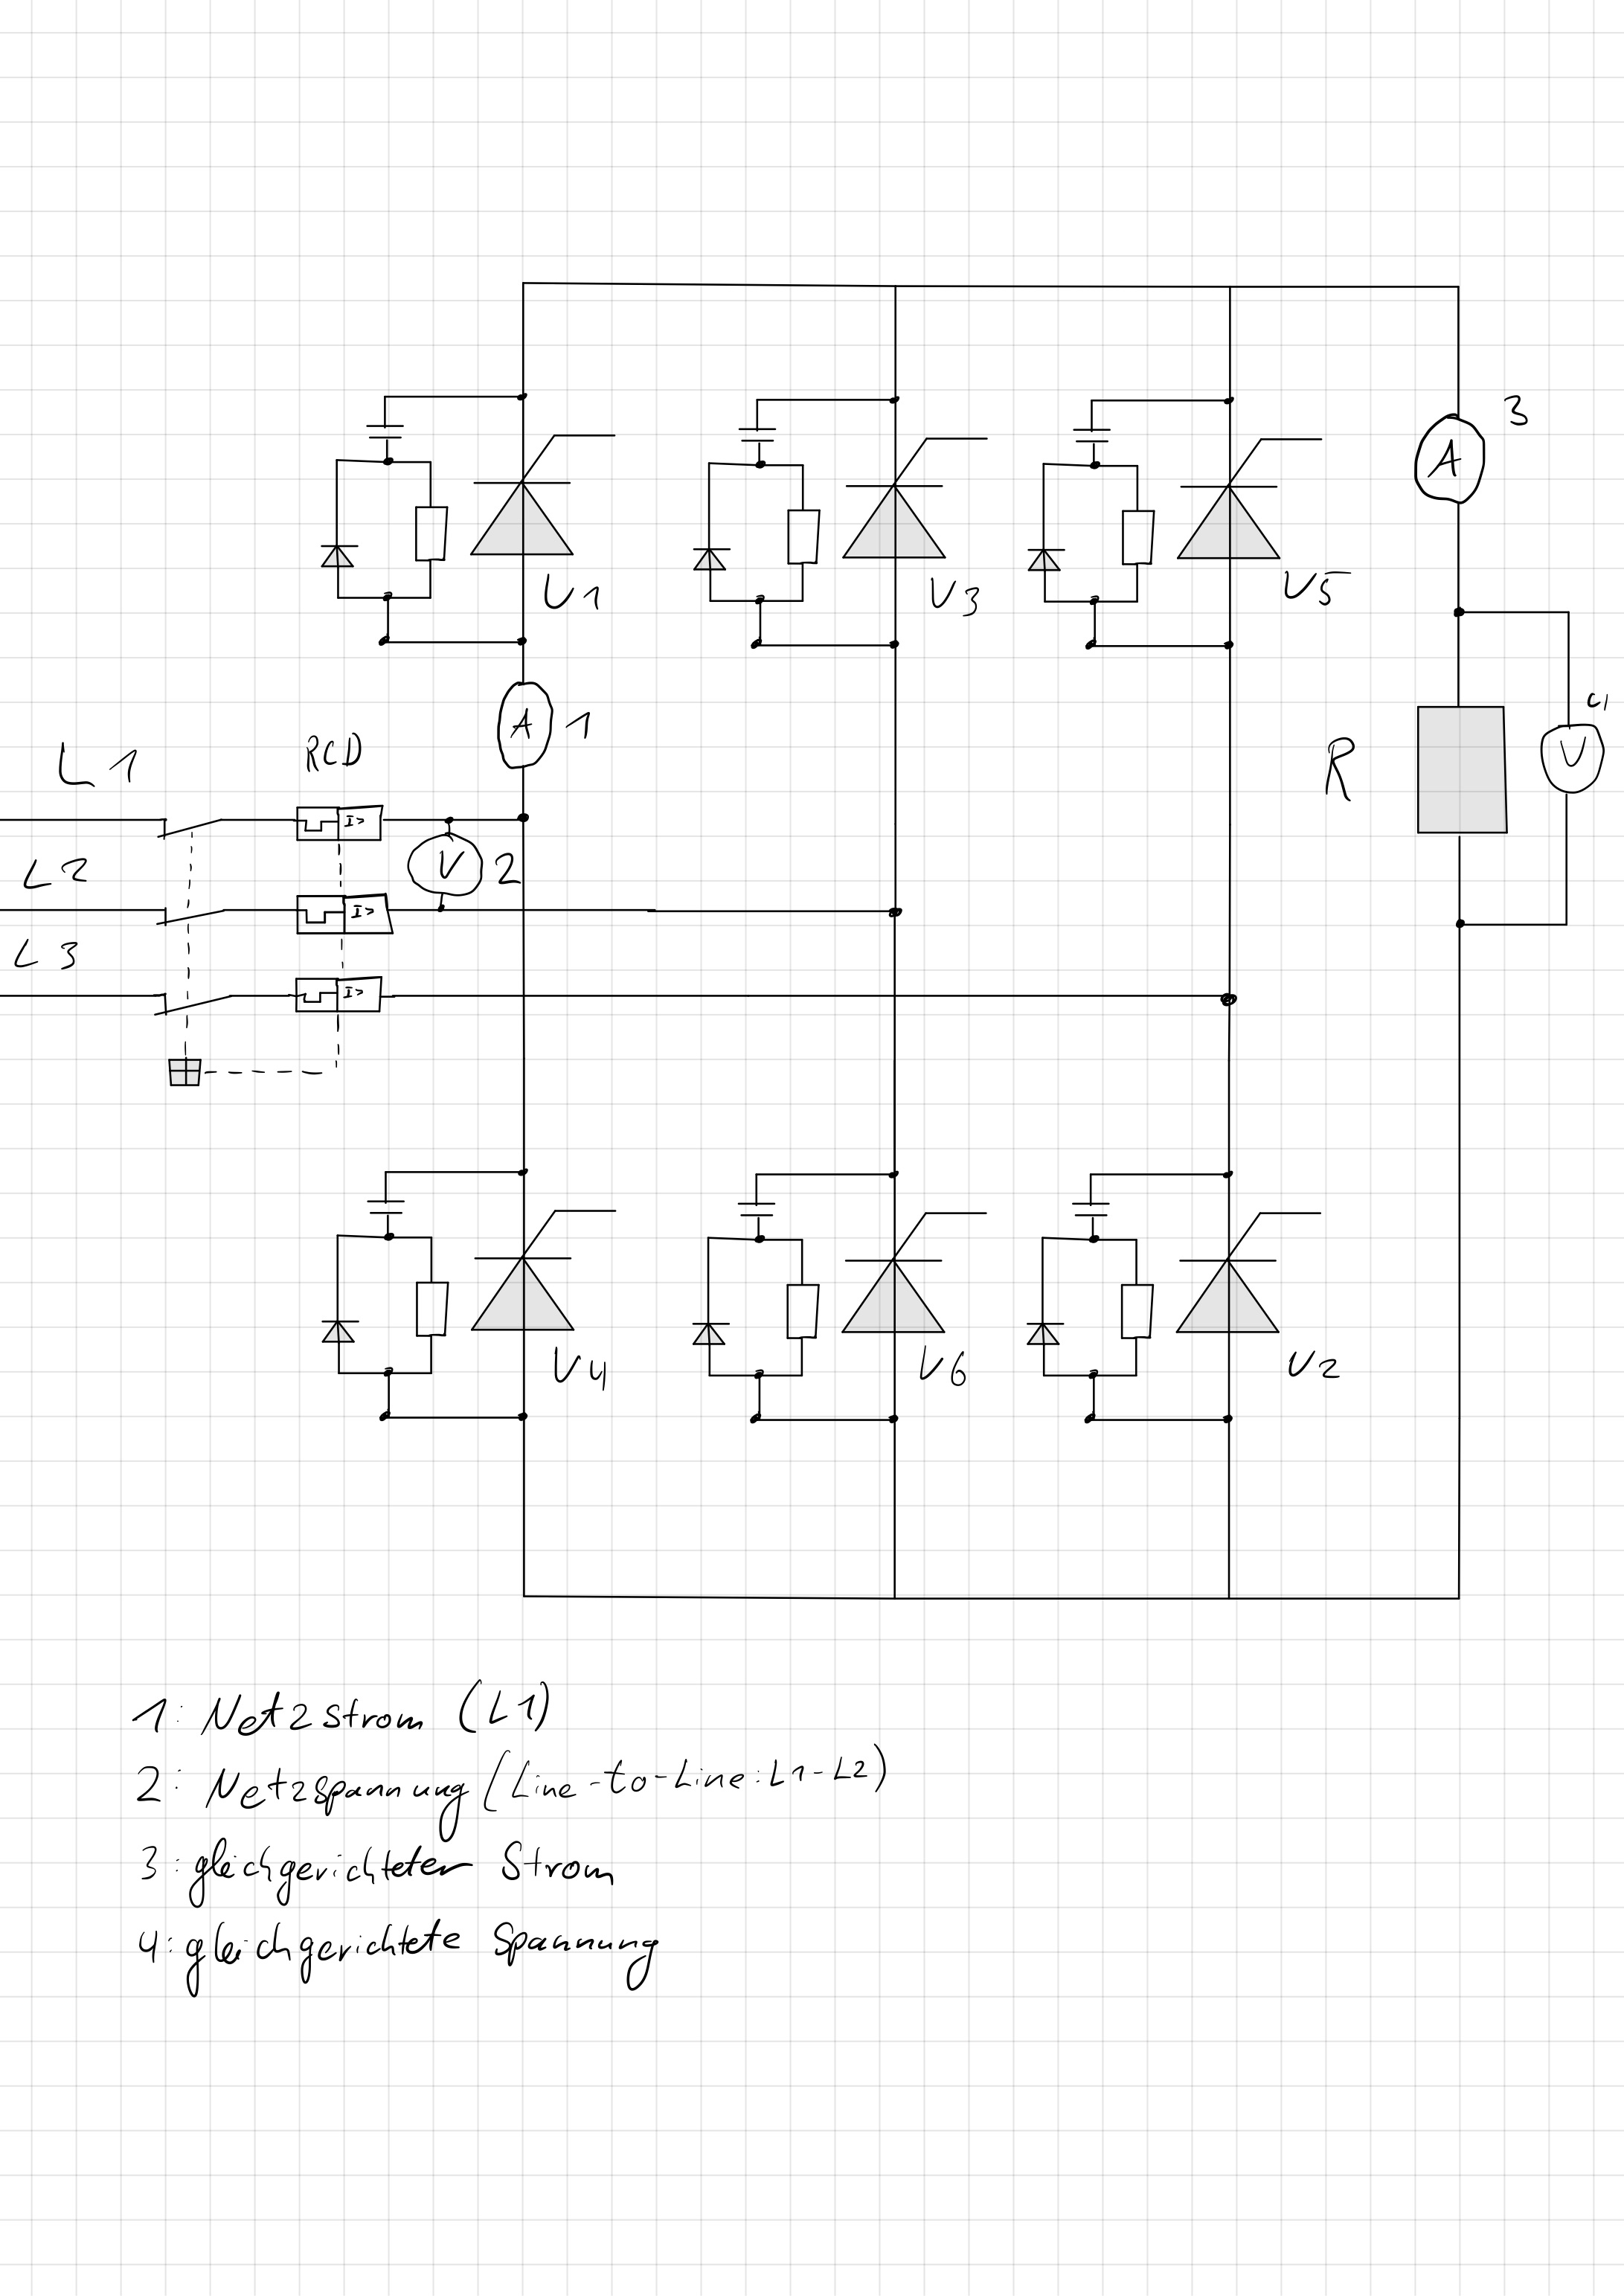
\includegraphics[width=0.8\textwidth]{../assets/images/GEP2/b6.jpg}
  \caption{Aufbau der B6-Brücke}
  \label{fig:b6}
\end{figure}

Zusätzlich wollen wir uns im Vorfeld überlegen, inwieweit wir sicherstellen können, dass die vorgegebenen Werte eingehalten werden können. Mit $U_{S} = 26V$ und $I_{d,max} = 2A$ können wir nun bei maximaler Aussteuerung der Schaltung, also bei $\alpha = 0^{^{\circ}}$, die maximale Spannung $$U_{di\alpha} = \frac{3\cdot \sqrt{2}}{\pi}\cdot U_{L} \cdot cos(0^{\circ}) = \frac{3\cdot \sqrt{2}}{\pi}\cdot 26V = 60.816V$$
berechnen. Um nun eine ohmsche Last zu berechnen, die die Schaltung in diesen Werten beschränkt rechnen wir

\begin{equation*}
  \label{eq:1}
  R_{L} = \frac{U_{di\alpha}}{I_{d,max}} = \frac{60,816V}{2A} = 30.4 \Omega
\end{equation*}

\section{Messreihe}

\subsection{Messung der Steuerspannung und der gleichgerichteten Spannung}

Wir wollen zunächst unseren Offset bei der Einstellung unseres Zündverzögerungswinkels ermitteln. Dabei stellen wir unsere Steuerspannung $U_{St} = 10V$ auf das Maximum ein und messen vom Nulldurchgang der Spannung $U_{21}$ zur ersten Zündung. Wir erhalten eine Verzögerung von $\Delta t = 3.68ms$, damit rechnen wir

\begin{equation*}
  \label{eq:2}
  \Delta\alpha = \Delta t \cdot 360^{\circ} \cdot \frac{1}{T} - 60^{\circ} = 3.68ms \cdot 360^{\circ} \cdot \frac{1}{20ms} - 60^{\circ} = 6,2^{\circ}
\end{equation*}

und erhalten damit den Winkel, den wir bei der minimalen Einstellung unseres Zündwinkeltransformators haben. Alle weiteren Messungen basieren dann auf diesem Offset. Der Bild auf dem Oszilloskop ist dann unten noch einmal dargestellt:

\begin{figure}[h]
  \centering
  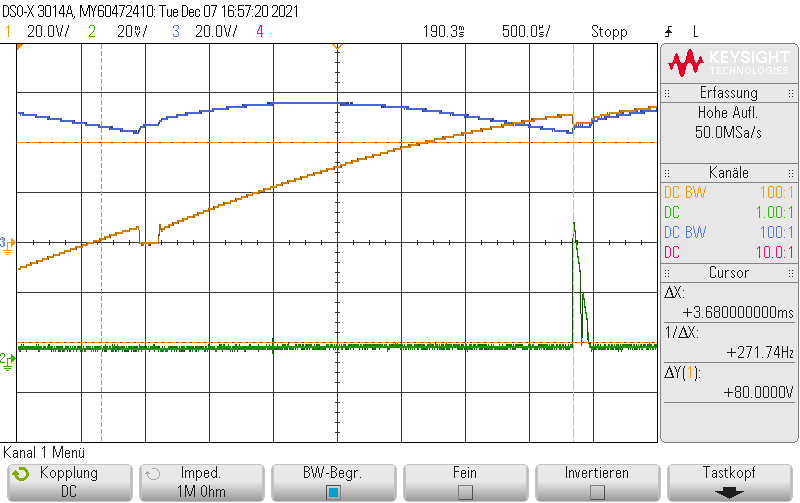
\includegraphics[width=\textwidth]{../assets/images/GEP2/startAngle.png}
  \caption{Startmessung des Winkels bei 10V}
  \label{fig:startAngle}
\end{figure}

\newpage

Wir wollen nun uns die Tabelle der Werte einmal anschauen:

\begin{table}[h]
  \centering
  \begin{tabular}{|c|c|c|}
    \hline
    $\alpha$ & $U_{St}$ & $U_{di\alpha}$ \\
    \hline
    $6,2^{\circ}$ & $56,6V$ & $10,008V$\\
    \hline
    $24,2^{\circ}$ &$53,01V$ & $9,058V$\\
    \hline
    $42,2^{\circ}$ &$44,1V$ & $8,059V$\\
    \hline
    $60,2^{\circ}$ & $31,6V$& $6,976V$\\
    \hline
    $78,2^{\circ}$ & $20,23V$& $6,131V$\\
    \hline
    $96,2^{\circ}$ & $8,96V$& $5,181V$\\
    \hline
    $114,2^{\circ}$ &$1,53V$ & $4,239V$\\
    \hline
    $132,2^{\circ}$ & $0,003V$& $3,3V$\\
    \hline
  \end{tabular}
  \caption{Messreihe der Steuerspannung und der gleichgerichteten Spannung im Bezug auf den Zündverzögerungswinkel}
  \label{tab:mess1}
\end{table}

Beispielhaft wollen wir uns dann auch das Oszilloskopbild mit den Spannungen $U_{21}$ und $U_{di\alpha}$ anschauen:

\begin{figure}[h]
  \centering
  \begin{subfigure}{.45\textwidth}
    \centering
    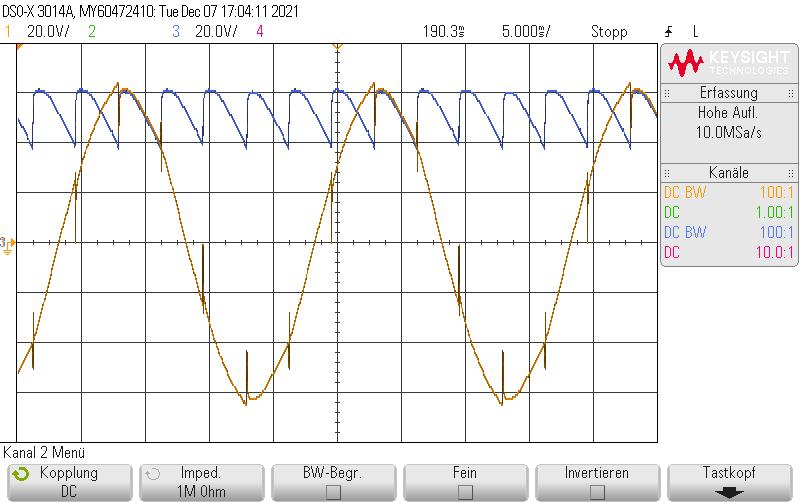
\includegraphics[width=\linewidth]{../assets/images/GEP2/31_Winkel242.png}
    \caption{Oszilloskopbild zur Messung 3.1 für den Winkel $24,2^{\circ}$}
  \end{subfigure}
  \begin{subfigure}{.45\textwidth}
    \centering
    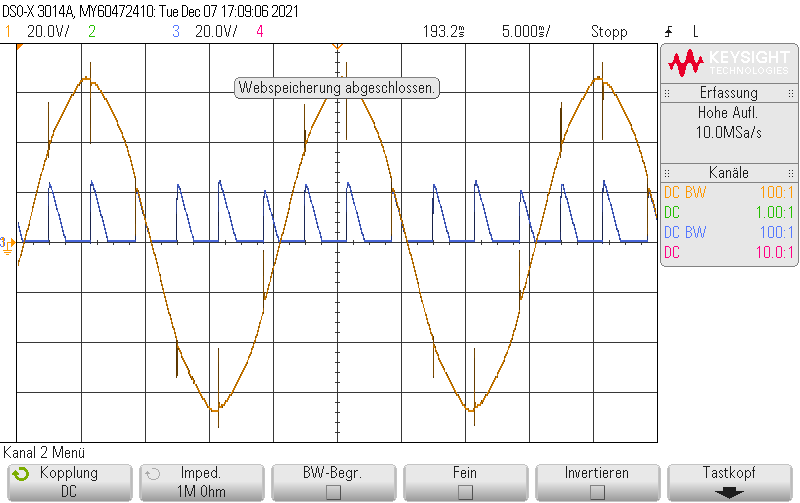
\includegraphics[width=\linewidth]{../assets/images/GEP2/31_Winkel962.png}
    \caption{Oszilloskopbild zur Messung 3.1 für den Winkel $96,2^{\circ}$}
  \end{subfigure}
  \label{fig:31_242}
  \caption{Beispielhafte Bilder vom Oszilloskop}
\end{figure}


\subsection{Messung von verschiedenen Kenndaten der B6-Brücke bei ohmscher Last}

Im nächsten Schritt wollen wir uns unter der vorher berechneten ohmschen Last, also eine Zusammenschaltung von drei $100\Omega$-Widerständen, verschiedene Kenndaten der B6-Brücke anschauen. Auch hier schauen wir uns die Werte in Abhängigkeit von dem Zündverzögerungswinkel $\alpha$ ausgehend von unserem Offset in $18^{\circ}$-Schritten an. Dabei entsprechen $18^{\circ}$ genau einer Milisekunde Verzögerung.

\begin{table}[h]
  \centering
  \begin{tabular}{|c|c|c|c|c|c|}
    \hline
    $\alpha$ & $P_{zu}$ & $U_{S}$ & $I_{L}$ & $I_{d}$ & $U_{di\alpha}$\\
    \hline
    $6,2^{\circ}$ & $33,4W$ & $1,39A$ & $25,24V$ & $1,67A$ & $56,3V$\\
    \hline
    $24,2^{\circ}$ & $28,8W$ & $1,297A$ & $25,36V$ & $1,55A$ & $52,2V$\\
    \hline
    $42,2^{\circ}$ & $19,75W$ & $1,073A$ & $25,67V$ & $1,26A$ & $42,34V$\\
    \hline
    $60,2^{\circ}$ & $10,77W$ & $0,7083A$ & $25,9V$ & $0,866A$ & $28,55V$\\
    \hline
    $78,2^{\circ}$ & $4,1W$ & $0,49A$ & $26,3V$ & $0,4512A$ & $15,14V$ \\
    \hline
    $96,2^{\circ}$ & $0,728W$ & $0,217A$ & $26,39V$ & $0,1577A$ & $5,204V$\\
    \hline
    $114,2^{\circ}$ & $0W$ & $0A$ & $26,6V$ & $0,04A$ & $0,33V$\\
    \hline
    $132,2^{\circ}$ & $0W$ & $0A$ & $26,5V$ & $0A$ & $0,08V$\\
    \hline
  \end{tabular}
  \caption{Kenndaten der B6-Brücke bei ohmscher Last in tabellarischer Form}
  \label{tab:mess2}
\end{table}


Um unsere Messungen graphisch zu überprüfen, schauen wir uns die dazugehörigen Oszilloskopbilder auch an. Wir erkennen, dass ein Erhöhung des Zündverzögerungswinkels mit dem Absinken der Leistung einhergeht. Das entspricht auch unseren Vorstellungen. Auch die gleichgerichtete Spannung ist proportional zum Zündverzögerungswinkel.

\begin{figure}[h]
  \centering
  \begin{subfigure}{.45\textwidth}
    \centering
    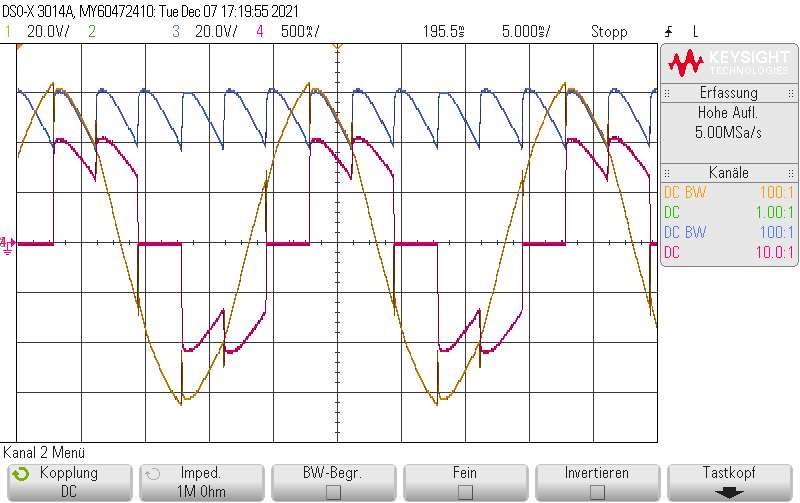
\includegraphics[width=\linewidth]{../assets/images/GEP2/32_Winkel242.png}
    \caption{Oszilloskopbild zur Messung 3.2 für den Winkel $24,2^{\circ}$}
  \end{subfigure}
  \begin{subfigure}{.45\textwidth}
    \centering
    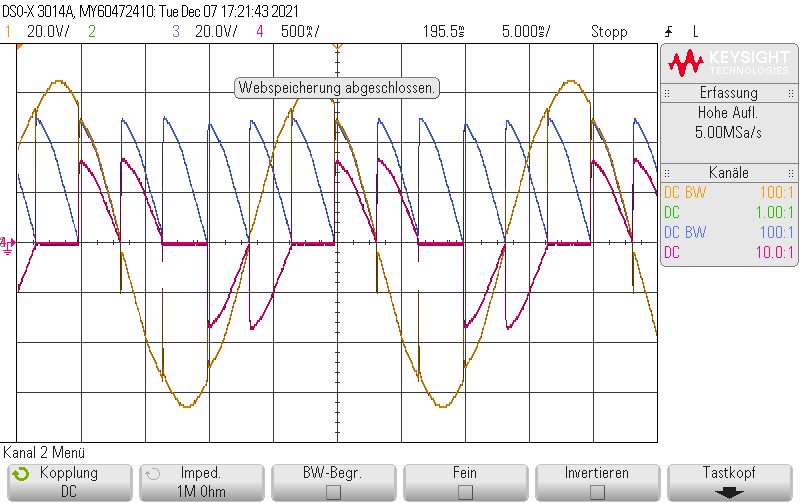
\includegraphics[width=\linewidth]{../assets/images/GEP2/32_Winkel602.png}
    \caption{Oszilloskopbild zur Messung 3.2 für den Winkel $60,2^{\circ}$}
  \end{subfigure}
  \label{fig:31_242}
  \caption{Zur Messung 3.2: Bilder vom Oszilloskop}
\end{figure}

\begin{figure}[h]
  \centering
  \begin{subfigure}{.45\textwidth}
    \centering
    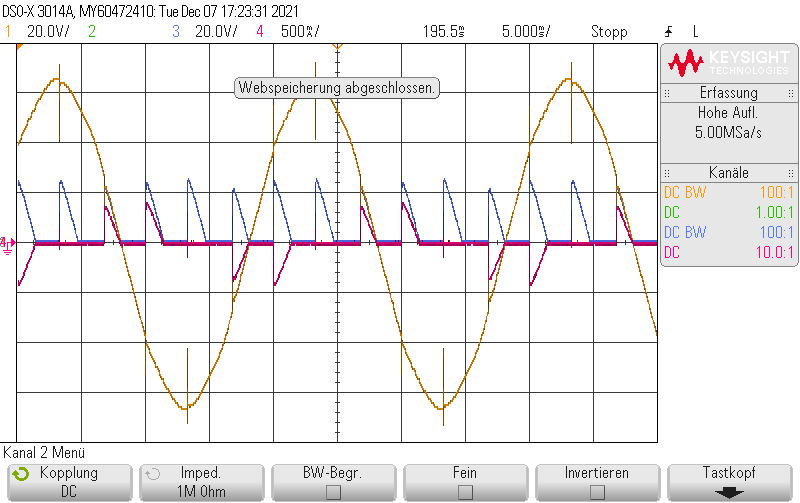
\includegraphics[width=\linewidth]{../assets/images/GEP2/32_Winkel962.png}
    \caption{Oszilloskopbild zur Messung 3.2 für den Winkel $96,2^{\circ}$}
  \end{subfigure}
  \begin{subfigure}{.45\textwidth}
    \centering
    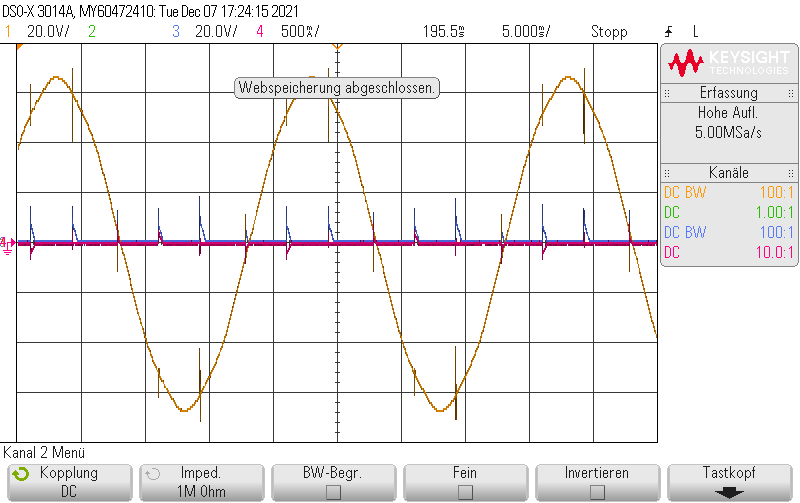
\includegraphics[width=\linewidth]{../assets/images/GEP2/32_Winkel1142.png}
    \caption{Oszilloskopbild zur Messung 3.2 für den Winkel $114,2^{\circ}$}
  \end{subfigure}
  \label{fig:31_242}
  \caption{Zur Messung 3.2: Bilder vom Oszilloskop}
\end{figure}

\newpage

\subsection{Messung von verschiedenen Kenndaten der B6-Brücke bei ohmsch-induktiver Last}

Wir wiederholen jetzt die Messung mit einer ohmsch-induktiven Last, indem wir zu dem Widerstand noch eine Induktivität mit $L = 50mH$ in Reihe schalten.

\begin{table}[h]
  \centering
  \begin{tabular}{|c|c|c|c|c|c|}
    \hline
    $\alpha$ & $P_{zu}$ & $U_{S}$ & $I_{L}$ & $I_{d}$ & $U_{di\alpha}$\\
    \hline
    $6,2^{\circ}$ & $33,15W$ & $1,347A$ & $25,96V$ & $1,626A$ & $58,17V$ \\
    \hline
    $24,2^{\circ}$ & $27,99W$ & $1,236A$ & $26,03V$ & $1,493A$ & $53,26V$\\
    \hline
    $42,2^{\circ}$ & $17,75W$ & $0,977A$ & $26,15V$ & $1,192A$ & $42,26V$ \\
    \hline
    $60,2^{\circ}$ & $7,49W$ & $0,636A$ & $26,42V$ & $0,77A$ & $27,6V$ \\
    \hline
    $78,2^{\circ}$ & $0,936W$ & $0,213A$ & $26,4V$ & $0,26A$ & $9,13V$\\
    \hline
    $96,2^{\circ}$ & $55mW$ & $5mA$ & $26,58V$ & $2,2mA$ & $-0,378VV$\\
    \hline
    $114,2^{\circ}$ & $0W$ & $0A$ & $26,48V$ & $0,7mA$ & $0V$ \\
    \hline
    $132,2^{\circ}$ & $0W$ & $0A$ & $26,58V$ & $0,21mA$ & $0V$ \\
    \hline
  \end{tabular}
  \caption{Kenndaten der B6-Brücke bei ohmsch-induktiver Last in tabellarischer Form}
  \label{tab:mess2}
\end{table}

\begin{figure}[h]
  \centering
  \begin{subfigure}{.45\textwidth}
    \centering
    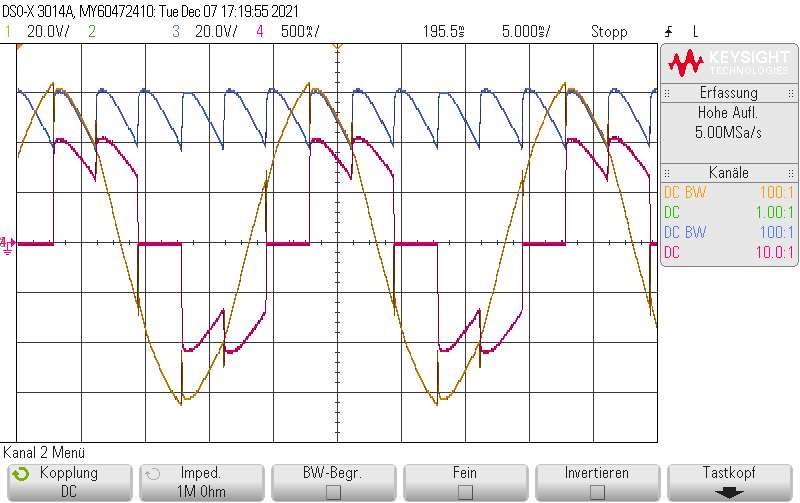
\includegraphics[width=\linewidth]{../assets/images/GEP2/32_Winkel242.png}
    \caption{Oszilloskopbild zur Messung 3.3 für den Winkel $24,2^{\circ}$}
  \end{subfigure}
  \begin{subfigure}{.45\textwidth}
    \centering
    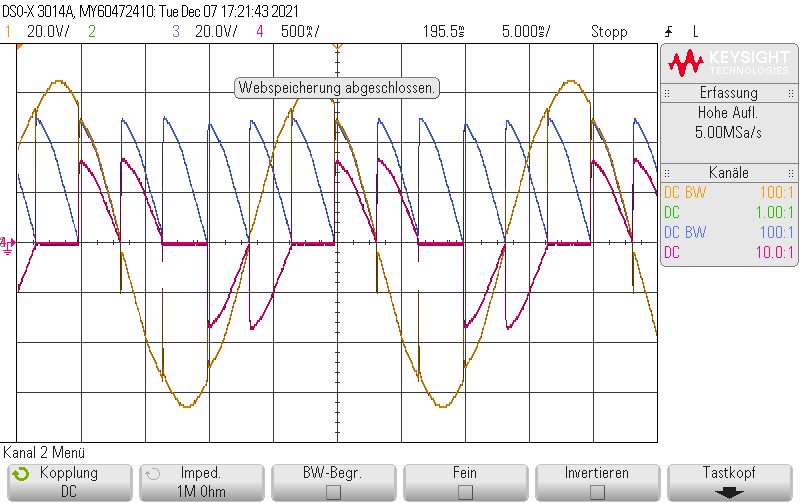
\includegraphics[width=\linewidth]{../assets/images/GEP2/32_Winkel602.png}
    \caption{Oszilloskopbild zur Messung 3.3 für den Winkel $60,2^{\circ}$}
  \end{subfigure}
  \label{fig:31_242}
  \caption{Zur Messung 3.3: Bilder vom Oszilloskop}
\end{figure}

\begin{figure}[h]
  \centering
  \begin{subfigure}{.45\textwidth}
    \centering
    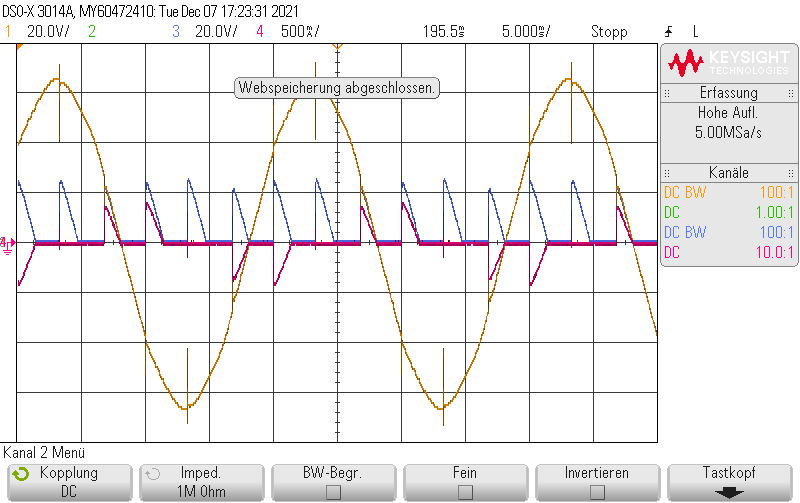
\includegraphics[width=\linewidth]{../assets/images/GEP2/32_Winkel962.png}
    \caption{Oszilloskopbild zur Messung 3.3 für den Winkel $96,2^{\circ}$}
  \end{subfigure}
  \begin{subfigure}{.45\textwidth}
    \centering
    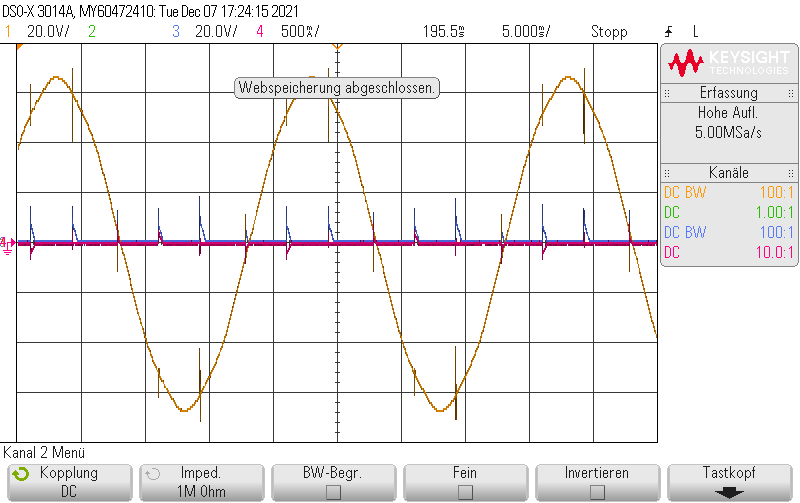
\includegraphics[width=\linewidth]{../assets/images/GEP2/32_Winkel1142.png}
    \caption{Oszilloskopbild zur Messung 3.3 für den Winkel $114,2^{\circ}$}
  \end{subfigure}
  \label{fig:31_242}
  \caption{Zur Messung 3.3: Bilder vom Oszilloskop}
\end{figure}


\section{Auswertung}

\subsection{Kennlinie von Steuerspannung zu Zündwinkel}
\label{sec:kennl-von-steu}

Aus der Messreihe 3.1 wollen wir die Kennlinie $\alpha = f(U_{St})$ erstellen:

\begin{figure}[h]
  \centering
  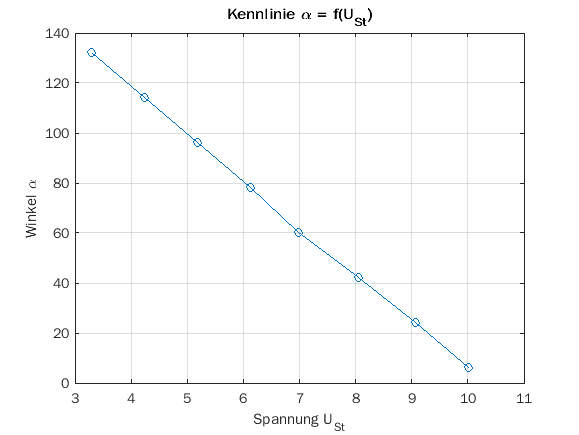
\includegraphics[width=\textwidth]{../assets/images/GEP2/alpha_ust.png}
  \caption{Kennlinie der Messung 3.1 mit Winkel zu Steuerspannung}
  \label{fig:alphaust}
\end{figure}

Wir erkennen einen anti-proportionalen Zusammenhang zwischen der Steuerspannung $U_{St}$ und dem Winkel $\alpha$. Dabei haben wir einen ungefähre Steigung von

\begin{equation*}
  m = \frac{\Delta y}{\Delta x} = \frac{6,2^{\circ} - 132,2^{\circ}}{10,008V - 3,3V} = \frac{-126^{\circ}}{6,7V} = -18,8 \frac{Grad}{V}
\end{equation*}

ermitteln können.

\subsection{Kennlinie von Winkel zu gleichgerichteten Spannung bei ohmscher Last}
\label{sec:kennlinie-von-winkel}

Als nächstes vergleichen wir die gemessenen Kennlinie von Winkel zu gleichgerichteter Spannung bei ohmscher Last zu der theoretischen Kennlinie:

\begin{figure}[h]
  \centering
  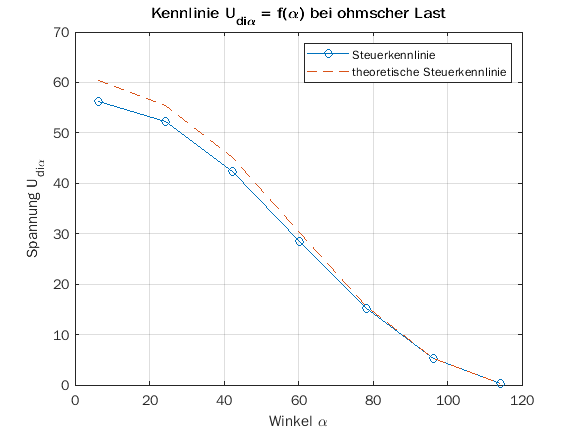
\includegraphics[width=\textwidth]{../assets/images/GEP2/udia_alpha_ohm.png}
  \caption{Gemessene zur theoretischen Kennlinie bei ohmscher Last}
  \label{fig:udiaalphaohm}
\end{figure}
Die gemessene und die theoretische Kennlinie haben am Anfang der Messung zunächst ein kleines Offset, der sich dann aber im Verlauf der Messung immer besser anpasst. Bei hohem Zündverzögerungswinkel sind die beiden Kennlinien beinahe identisch.
Zur Berechnung der theoretischen Kennlinie sollte bedacht werden, dass eine B6-Brücke bei rein ohmscher Last ab $\alpha > 60^{\circ}$ in einen lückenden Betrieb geht. Es gilt:
\begin{equation*}
  a_{th} = \begin{cases}
    cos(\alpha) & 0^{\circ}\leq\alpha\leq 60^{\circ}\\
    1 + \frac{cos(\alpha)}{2} - \frac{\sqrt{3}\cdot sin(\alpha)}{2} & 60^{\circ}\leq\alpha\leq 120^{\circ}\\
  \end{cases}
\end{equation*}
mit der Gleichung
\begin{equation}
  \label{eq:3}
  U_{di\alpha, th} = \frac{3\cdot\sqrt{2}}{\pi}\cdot U_{L}\cdot a_{th}
\end{equation}


\subsection{Kennlinie von Winkel zu gleichgerichteter Spannung bei ohmsch-induktiver Last}
\label{sec:kennlinie-von-winkel-1}
Wir wiederholen die Analyse jedoch diesmal bei ohmsch-induktiver Last. Die Kennlinien sehen dabei folgendermaßen aus:

\begin{figure}[h]
  \centering
  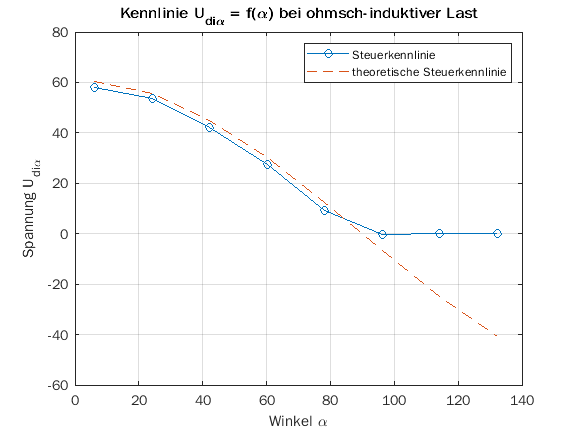
\includegraphics[width=\textwidth]{../assets/images/GEP2/udia_alpha_induk.png}
  \caption{Gemessene zur theoretischen Kennlinie bei ohmsch-induktiver Last}
  \label{fig:udiaalphainduk}
\end{figure}
Auch hier berechnen wir die theoretische Steuerkennlinie über

\begin{equation*}
  \label{eq:4}
  \begin{array}{ll}
    a_{th} = cos(\alpha) & 0^{\circ} \leq\alpha\leq 120^{\circ}\\
  \end{array}
\end{equation*}

mit der Gleichung (\ref{eq:3}).

Diese Kennlinien sind am Beginn der Messung ziemlich nah beieinander, driften jedoch ab einem Winkel von ca. $\alpha = 78,2^{\circ}$ stark voneinader ab. Die theoretische Kennlinie geht dabei auch weit in den negativen Bereich über. Dies lässt sich auf die Speichereigenschaft der Spule zurückführen. In der mathematischen Berechnung erreicht der $cos(\alpha)$ für $\alpha > 90^{\circ}$ den negativen Bereich, weshalb die berechnete Kennlinie hier in den negativen Bereich übergeht.

\subsection{Scheinleistung und Leistungsfaktor}
\label{sec:sche-und-leist}

Im letzten Teil der Auswertung wollen wir nun die Scheinleistung und den daraus resultierenden Leistungsfaktor berechnen. Die Scheinleistung berechnet sich über

$$S = U_{1N}\cdot I_{L}$$

Für den Leistungsfaktor rechnen wir

\[
  \begin{array}{ll}
    \lambda = \frac{P_{zu}}{S} & \text{mit $P_{zu}$ als Wirkleistung}\\
  \end{array}
\]
Die Größen für die Berechnung der beiden Werte können wir aus den Messungen 3.2 und 3.3 entnehmen.

\begin{table}[h]
  \centering
  \begin{subtable}{.5\linewidth}
    \centering
    \caption{bei ohmscher Last}
    \begin{tabular}{|c|c|c|}
      $S$ & $P_{zu}$ & $\lambda$ \\
      $35,0836VA$ & $33,4W$ & $0,952$\\
      $32,891VA$ & $28,8W$ & $0,8756$\\
      $27,5439VA$ & $19,75W$ & $0.717$\\
      $18,345VA$ & $10.77W$ & $0.5871$\\
      $12,887VA$ & $4,1W$ & $0,3182$\\
      $5.7266VA$ & $0.728W$ & $0.1271$\\
      $0VA$ & $0W$ & $-$\\
      $0VA$ & $0W$ & $-$\\
    \end{tabular}
  \end{subtable}
  \begin{subtable}{.5\linewidth}
    \centering
    \caption{bei ohmsch-induktiver Last}
    \begin{tabular}{|c|c|c|}
      \hline
      $S$ & $P_{zu}$ & $\lambda$ \\
      \hline
      $34,9681VA$ & $33,15W$ & $0,948$\\
      \hline
      $32,1731VA$ & $27.99W$ & $0,87$\\
      \hline
      $25,5485VA$ & $17,75W$ & $0.6948$\\
      \hline
      $16,8031VA$ & $7,49W$ & $0,4458$\\
      \hline
      $5,6232VA$ & $0.936W$ & $0,1665$\\
      \hline
      $0,1329VA$ & $0,055W$ & $0.4138$\\
      \hline
      $0VA$ & $0W$ & $-$\\
      \hline
      $0VA$ & $0W$ & $-$\\
      \hline
    \end{tabular}
  \end{subtable}
  \caption{Tabelle der Scheinleistung und des Leistungsfaktors}
  \label{tab:scheinfak}
\end{table}


\section{Konklusion}
\label{sec:konklusion}

Aus dem Labor konnten wir das Verhalten der B6-Brücke besser verstehen, indem wir verschiedene Schaltvorgänge und Verhalten der Schaltung genauer untersucht haben und selbst mit der Schaltung arbeiten konnten. Wir haben viele Zusammenhänge, die wir in der Vorlesung bereits behandelt haben, besser verinnerlichen können.


\end{document}
